\section{Built-in Grids}

The gridgen library includes some built-in grids
for some particularly difficult geometries that are
expected to be used frequently. 
This section will outline sketches (and
additional documentation ?) of the construction of each grid.


%
\begin{figure}[h]
\vspace{0.3cm}
   \fontxfig
   \psfrag{e1}[t][t][1][0]{$\varepsilon_1$}
   \psfrag{e2}[t][t][1][0]{$\varepsilon_2$}
   \psfrag{e3}[l][l][1][0]{$\varepsilon_3$}
   \psfrag{e4}[t][t][1][0]{$\varepsilon_4$}
   \psfrag{N1}[][][1][0]{$N_1$}
   \psfrag{N2}[][][1][0]{$N_2$}
   \psfrag{r1}[][][1][0]{$r_1$}
   \psfrag{r2}[][][1][0]{$r_2$}
   \psfrag{r3}[][][1][0]{$r_3$}
   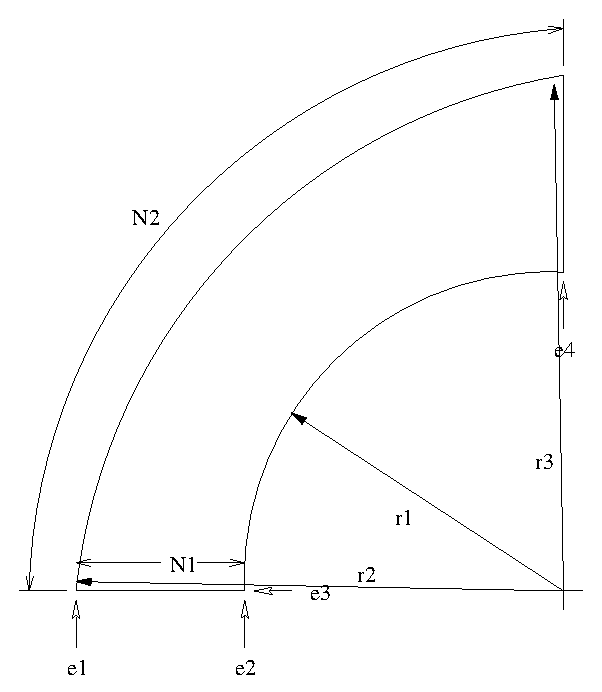
\includegraphics[width=3.0in]{gridBlunt2D.eps}
\caption{GridBlunt2D: constructing a 2D blunt body}
\label{fig:gridBlunt2D}
\end{figure}
%


%
\begin{figure}[h]
\vspace{0.3cm}
   \fontxfig
   \psfrag{e1}[][][1][0]{$\varepsilon_1$}
   \psfrag{e2}[bl][bl][1][0]{$\varepsilon_2$}
   \psfrag{t1}[r][r][1][0]{$\theta_1$}
   \psfrag{t2}[r][r][1][0]{$\theta_2$}
   \psfrag{L1}[t][t][1][0]{$L_1$}
   \psfrag{L2}[t][t][1][0]{$L_2$}
   \psfrag{L3}[br][br][1][0]{$L_3$}
   \psfrag{L4}[][][1][0]{$L_4$}
   \psfrag{L5}[t][t][1][0]{$L_5$}
   \psfrag{L6}[b][b][1][0]{$L_6$}
   \psfrag{L7}[b][b][1][0]{$L_7$}
   \psfrag{N1}[b][b][1][0]{$N_1$}
   \psfrag{N2}[b][b][1][0]{$N_2$}
   \psfrag{N3}[][][1][0]{$N_3$}
   \psfrag{N4}[][][1][0]{$N_4$}
   \psfrag{N5}[b][b][1][0]{$N_5$}
   \psfrag{N6}[t][t][1][0]{$N_6$}
   \psfrag{dz1}[b][b][1][0]{$\Delta \zeta_1$}
   \psfrag{dz2}[b][b][1][0]{$\Delta \zeta_2$}
   \psfrag{dz3}[bl][bl][1][0]{$\Delta \zeta_3$}
   \psfrag{dz4}[br][br][1][0]{$\Delta \zeta_4$}
   \psfrag{dz5}[b][b][1][0]{$\Delta \zeta_5$}
   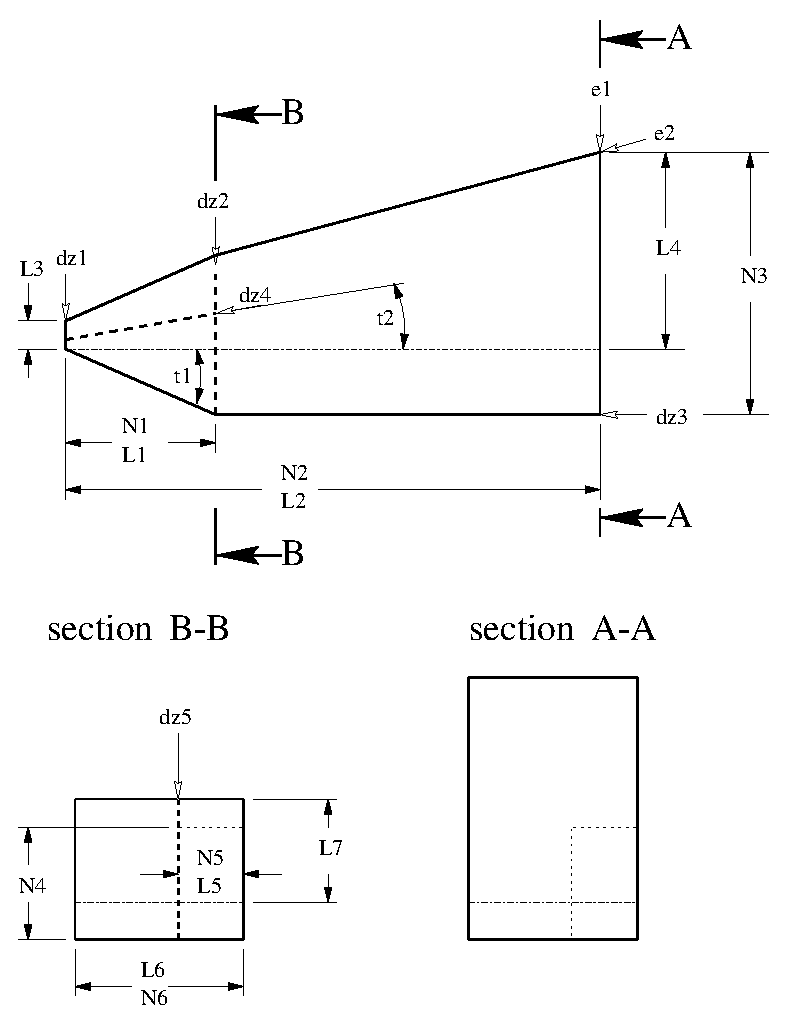
\includegraphics[width=6.0in]{gridRamp3D.eps}
\caption{GridRamp3D: constructing a 3D Ramp injector}
\label{fig:gridRamp3D}
\end{figure}
%

%
\begin{figure}[h]
\vspace{0.3cm}
   \fontxfig
   \psfrag{e1}[][][1][0]{$\varepsilon_1$}
   \psfrag{e2}[bl][bl][1][0]{$\varepsilon_2$}
   \psfrag{t1}[r][r][1][0]{$\theta_1$}
   \psfrag{t2}[r][r][1][0]{$\theta_2$}
   \psfrag{L1}[t][t][1][0]{$L_1$}
   \psfrag{L2}[t][t][1][0]{$L_2$}
   \psfrag{L3}[br][br][1][0]{$L_3$}
   \psfrag{L4}[][][1][0]{$L_4$}
   \psfrag{L5}[t][t][1][0]{$L_5$}
   \psfrag{L6}[b][b][1][0]{$L_6$}
   \psfrag{L7}[b][b][1][0]{$L_7$}
   \psfrag{L8}[b][b][1][0]{$L_8$}
   \psfrag{L9}[b][b][1][0]{$L_9$}
   \psfrag{L10}[b][b][1][0]{$L_{10}$}
   \psfrag{N1}[b][b][1][0]{$N_1$}
   \psfrag{N2}[b][b][1][0]{$N_2$}
   \psfrag{N3}[][][1][0]{$N_3$}
   \psfrag{N4}[][][1][0]{$N_4$}
   \psfrag{N5}[b][b][1][0]{$N_5$}
   \psfrag{N6}[t][t][1][0]{$N_6$}
   \psfrag{N7}[t][t][1][0]{$N_7$}
   \psfrag{N8}[t][t][1][0]{$N_8$}
   \psfrag{dz1}[b][b][1][0]{$\Delta \zeta_1$}
   \psfrag{dz2}[b][b][1][0]{$\Delta \zeta_2$}
   \psfrag{dz3}[bl][bl][1][0]{$\Delta \zeta_3$}
   \psfrag{dz4}[br][br][1][0]{$\Delta \zeta_4$}
   \psfrag{dz5}[b][b][1][0]{$\Delta \zeta_5$}
   \psfrag{dz6}[b][b][1][0]{$\Delta \zeta_6$}
   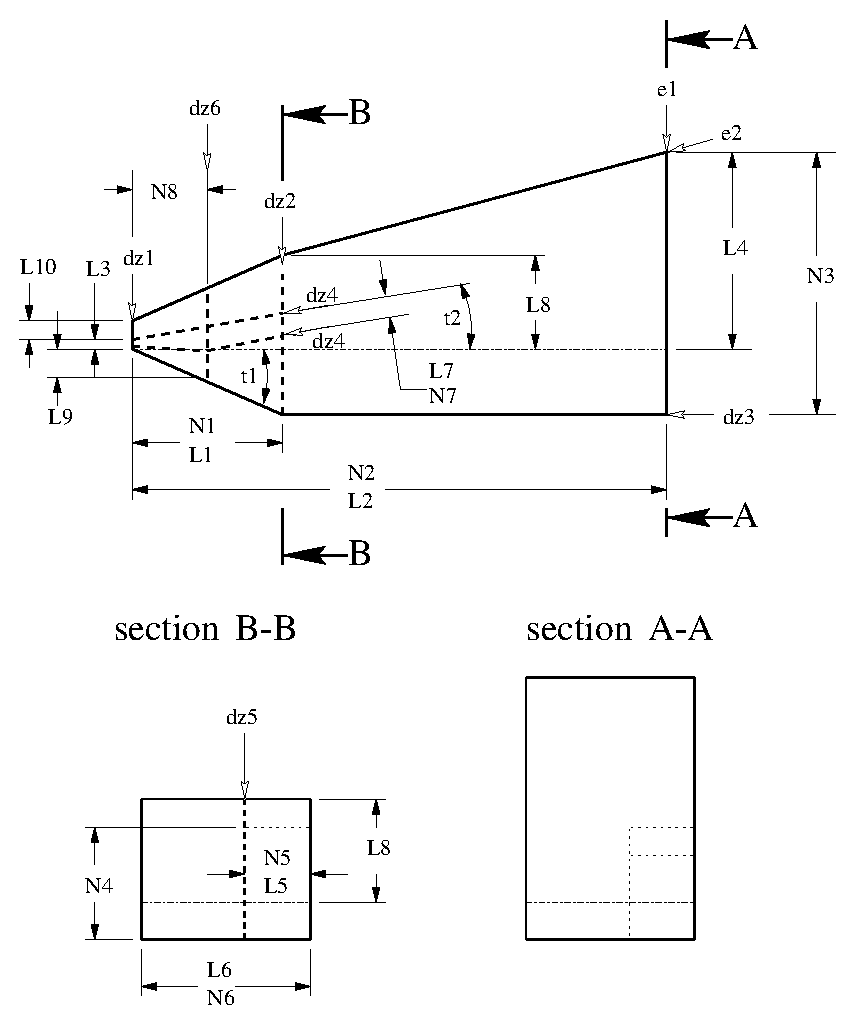
\includegraphics[width=6.0in]{gridCant3D.eps}
\caption{GridCant3D: constructing a 3D Cantilevered injector}
\label{fig:gridCant3D}
\end{figure}
%

